\documentclass[article]{IEEEtran}
\usepackage[brazilian]{babel}
\usepackage[utf8]{inputenc}
\usepackage{cite}
\usepackage{geometry}
\usepackage{graphicx}
\usepackage{amsmath}
\graphicspath{{./images/}}
\usepackage{float}

\begin{document}

%
% paper title
% Titles are generally capitalized except for words such as a, an, and, as,
% at, but, by, for, in, nor, of, on, or, the, to and up, which are usually
% not capitalized unless they are the first or last word of the title.
% Linebreaks \\ can be used within to get better formatting as desired.
% Do not put math or special symbols in the title.
\title{Utilização de fibras ópticas em sistemas de telecomunicação}



% author names and affiliations
% transmag papers use the long conference author name format.

\author{
	Felipe C. S. Santos,
	\and
	Thiago K. Lago
	
\IEEEauthorblockA{Universidade Federal do Rio de janeiro \\ 
	Escola Polit\'{e}cnica \\
	Departamento de Engenharia Eletrônica}
}



\IEEEtitleabstractindextext{
\begin{abstract}

\end{abstract}
\begin{IEEEkeywords}
Telecomunicações, fibras ópticas, optoeletrônica
\end{IEEEkeywords}}



% make the title area
\maketitle

\IEEEdisplaynontitleabstractindextext
As fibras ópticas tem diversas finalidades, sendo uma das mais importantes a utilização em telecomunicações. O avanço das tecnologias de fabricação, modulação e também instrumentação tem tornado cada vez mais viável a utilização das mesmas para transmissões de dados a grandes distâncias com altas taxas de bits. Busca-se através deste paper mostrar o processo de escolha de dimensionamento de uma rede baseada em componentes óticos.
\IEEEpeerreviewmaketitle



\section{Introducão}

\section{Construção da fibra}
Comentar sobre os materiais que são construídos, as janelas de transmissão, os tipos de dispersão, custo-benefício de cada uma delas.

\section{Componentes óticos}
Comentar sobre alguns componentes óticos utilizados como fbg para filtragem dos sinais e amplificadores ópticos

\section{Instrumentros de Medida}
É necessário se preocupar também com a qualidade do sinal recebido e a integridade da fibra óptica. Para isto são utilizados alguns equipamentos que permitem fazer a inspeção das mesmas e analisar o sinal recebido.

Ao instalar uma fibra de grande comprimento, a mesma pode sofrer avarias durante o percurso, prejudicando a recepção do sinal. Outro fator que pode ser determinante na qualidade do sinal recebido é a presença de emendas entre os pedaços das fibras. Existem alguns instrumentos utilizados para resolver este problema. Um deles é o OTDR (\textit{Optical Time Domain Reflectometer}).

\subsection{OTDR}
O \textbf{\textit{OTDR}}  utiliza o efeito de retroespalhamento (\textbf{\textit{backscattering}}) dos raios de luz durante a passagem dos sinais luminosos pela fibra óptica. Assim sendo, torna-se possível medir a atenuação do sinal conforme a distância, assim como visto \cite{FOA}

Esse instrumento possui um laser que emite luz em uma frequência pré-determinada e através da diferença de tempo e da potência do sinal medido após o retroespalhamento é possível determinar a relação entre o sinal recebido e a reflexão em uma dada distância de fibra, assim como visto na figura \ref{fig:otdr_esquematico}. Com isso se torna possível fazer uma inspeção na fibra sem a necessidade de retirar-la do local onde está instalada.


\begin{figure}[H]
	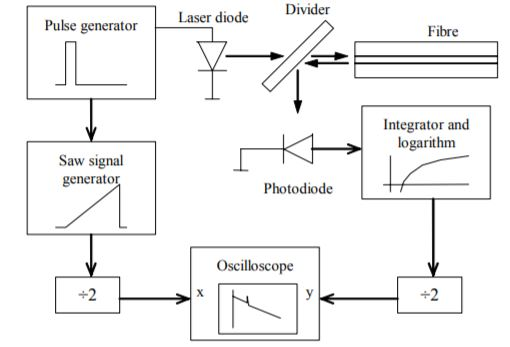
\includegraphics[width=0.5\textwidth]{images/OTDR_esquematico.JPG}
	\caption{Experimento de bancada com OTDR}
	\label{fig:otdr_esquematico}
\end{figure}

O equipamento deve ser conectado conforme a figura [\ref{fig:otdr_teste}], sendo que o cabo de teste pode ter comprimento de alguns quilômetros e ainda sim  pode ser possível realizar a análise com certa clareza. Após uma certa distância, que depende da potência do sinal emitido, da atenuação e reflexão sofrida durante o percurso, o sinal fica num nível comparável ao ruído, conforme visto à esquerda da figura \ref{fig:otdr_teste}:
\begin{figure}[H]
	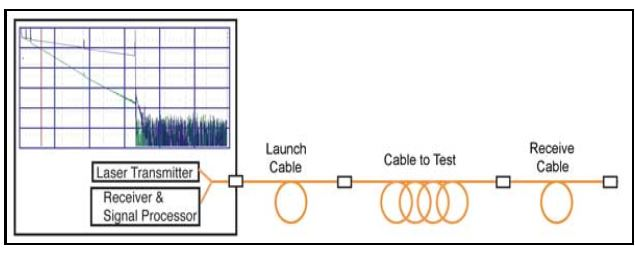
\includegraphics[width=0.5\textwidth]{images/OTDR_teste.JPG}
	\caption{Experimento de bancada com OTDR}
	\label{fig:otdr_teste}
\end{figure}

Uma maneira de aumentar a distância que o sinal chega sem ser muito atrapalhado por ruído é diminuindo o comprimento de onda do laser utilizado na inspeção da fibra. Todavia, isto faz com que a resolução do caminho percorrido diminua, sendo assim, obtêm-se menos informação sobre o caminho percorrido pelo sinal. Cabe ao operador do OTDR ajustar o equipamento de forma a obter o melhor compromisso entre distância e resolução, assim como visto em \cite{OTDR_LAB}.

A inclinação da curva na parte linear indica o coeficiente de atenuação da fibra (db/km). Quanto menor a inclinação, mais longe consegue-se transmitir um sinal até que ele chegue à uma razão sinal ruído (\textbf{SNR}) mínima pré-determinada.

Ao utilizar o equipamento para medir a atenuação do sinal conforme a distância da fibra, pode-se observar um gráfico similar ao visto na figura \ref{fig:OTDR_grafico}:
\begin{figure}[H]
	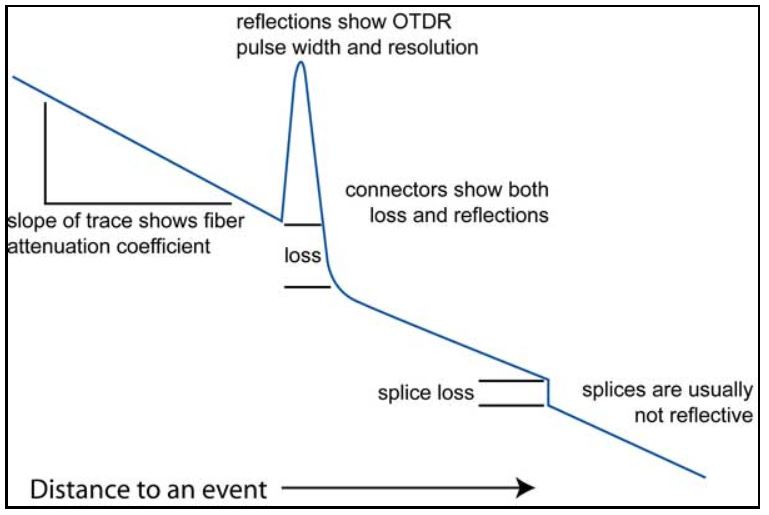
\includegraphics[width=0.5\textwidth]{images/OTDR_grafico.JPG}
	\caption{Experimento de bancada com OTDR}
	\label{fig:OTDR_grafico}
\end{figure} 

Busca-se observar os pontos onde existem descontinuidades na reta de potência do sinal por distância. Estes pontos podem indicar a utilização de um conector mecânico, solda ou até mesmo um rompimento na fibra. Quando a conexão entre fibras é bem feita, a observa-se pouca atenuação no sinal, sendo que a solda bem feita atenua menos que um conector mecânico. Caso observe-se que a inclinação cai bruscamente e o nível do sinal fica próximo ao ruído, pode-se suspeitar de uma fibra rompida ou de uma conexão mal feita.

Existem OTDRs com diferentes finalidades. Antes de fazer a compra do mesmo, necessita-se avaliar o resultado que deseja-se obter com o equipamento. Algumas das perguntas que podem ser feitas são: Há necessidade de ser portátil? Precisa ter bateria? Se precisar, esta deseja-se que esta dure por longo período? A tela precisa ser grande? Qual distância máxima da fibra que desejá-se trabalhar? Qual resolução que se espera nos resultados obtidos? Conforme a pesquisa de preço feito no site mercado livre no dia 30/11/2018 \cite{M_LIVRE}, um OTDR novo pode variar entre R\$3.981, e R\$35.000.

\section{Espectrômetro}


\section{Conclusão}


\bibliographystyle{ieeetr}
\bibliography{citations}

\end{document}



